\section{Routing, feedback and stopping}
\label{sec:routing}

The state record of \cref{sec:records} holds every value that the planning agent keeps between
steps. This section shows how the merged record selects the next step, sends execution back to an
earlier location when work has to be redone, and ends the run. Every return to an earlier location
adds work to the run, and every ending is later read from the trace, so we need to know what these
mechanisms guarantee. We ask when a run is certain to stop, and what its trace can establish about
how it stopped.

\subsection{Routing functions and conditional edges}
\label{sec:routing-functions}

After a node runs, the routing function attached to it reads the merged record and selects the next
control location. As in Lecture~2 and \cref{sec:machines}, a routing function is code that we write:
it reads the state and returns the name of the node that runs next. In the planning agent, every
node except \demoref{validate} has a routing function. The edge from \demoref{validate} to
\demoref{END} is unconditional, so the run always ends after the \demoref{validate} node. Its
status is the verdict, or \demoref{budget\_exhausted} when the admission check stopped the
validator's call.

A step in which the model is called passes through a cycle of proposal, record and decision:
\bi
\item \textbf{Proposal.} The model emits a tool call, a plan, a candidate patch or a verdict. We
call this output a proposal because it decides nothing by itself.
\item \textbf{Record.} The runtime merges the node's partial update into the state record, using
each field's reducer (\cref{sec:records}). It also appends events to the trace that describe what
happened.
\item \textbf{Decision.} The routing function tests fields of the merged record. The guards and
limits that the programmer wrote determine which destination it returns. After the
\demoref{validate} node, the destination is always \demoref{END}. The status records the verdict, or
\demoref{budget\_exhausted} when the admission check stopped the call before a verdict.
\ei

Lecture~2 described a conditional edge as an edge that is taken only when a predicate over the state
selects it. In the vocabulary of \cref{sec:machines}, each conditional edge is one transition, and
its predicate is that transition's guard, a condition on the merged record. All the conditional
edges that leave one control location share one routing function. The function tests their guards
and returns one destination.

A guard can test any field of the merged record. This includes the value the latest step wrote,
such as the model's reply. It also includes values retained from earlier steps, such as the number
of model calls made so far. Another example is the handoff field \demoref{failed\_step}, which the
tools node sets on the first stall and the routing function after \demoref{tools} tests
(\cref{sec:records}). A routing
decision therefore depends on the history of the run, as far as the record retains it.

A routing function stops the run by returning \demoref{END}. The returned name says only that the
run is over. The \demoref{status} field of the record says why it stopped.

The trace records routing decisions as routing events (Lecture~2). It has no routing event for the
moves from \demoref{tools} and from \demoref{plan} to the controller, which are inferred
(\cref{sec:machines}). A routing event's \demoref{by} field names the source of the value that the
guard tested:
\bi
\item \textbf{By the model.} The field holds \demoref{model} when the tested value came from the
model's output, for example the presence of a tool call in its reply.
\item \textbf{By the runtime.} The field holds \demoref{runtime} when the tested value came from a
check, such as a failed submit check, or from a limit, such as an exhausted budget. It also holds
\demoref{runtime} for a default, a value that the runtime supplies in place of a model output.
\ei
In both cases the programmer defined the edge and its guard. The \demoref{by} field records who
supplied the tested value. It does not record who wrote the rule that tested it.

The routing function after the controller, \demoref{after\_controller}, shows how the model's reply
affects routing at that location. \Cref{sec:machines} gives its code in \cref{lst:machines-transition},
and it is the same function as in the reactive loop of Lecture~2, Section~3. It makes two tests, in
this order:
\bi
\item \textbf{The status test.} If the status is no longer \demoref{running}, a limit or a check has
stopped the run, and the function returns \demoref{END}. The runtime supplied the tested value.
\item \textbf{The tool-call test.} For an active run, the function returns \demoref{tools} if the
last reply contains tool calls, and \demoref{submit} otherwise. The model supplied the tested
value.
\ei

The function reads the \demoref{tool\_calls} field of the reply. It never reads the reply's text.
Suppose that an active run receives a reply that claims the patch is correct and also requests a
tool. The run goes to \demoref{tools}, because the reply contains a tool call, and the claim in
the text has no effect. At the controller, the model can change the path of a run only by including
tool calls in its reply or leaving them out. The guards we wrote decide where each choice leads.

\subsection{The same graph, different paths}
\label{sec:routing-paths}

The compiled graph fixes which transitions are possible, and the record decides which of them a run
takes. As in Lecture~2, the graph is compiled once, before any alert is read, and every run executes
the same compiled graph. During a run, each routing function uses the current record to select a
destination.

Every visit to a control location that has a routing function leads to a new routing decision. A
run can visit the controller many times. At each visit, the routing function after the controller
runs again on the record as it stands after that visit. The same location can therefore lead to
different destinations within one run.

The computation tree of \cref{sec:machines} shows this. The tree has a separate node for each visit
to a control location. Each tree node represents the configuration of that visit: the location
together with the values in the record. In the recorded run of \cref{sec:machines}, the first four
visits to the controller produced replies with tool calls and routed to \demoref{tools}. The
fifth produced a reply without one and routed to \demoref{submit}. The location, the graph and the
routing function were the same at every visit. Only the record differed.

The same tree also contains the branches that this run did not take. At \demoref{submit}, a failed
check would have sent the run back to the controller. At \demoref{validate}, the validator could
have rejected the patch. At a later visit to the controller, the budget could have run out. The
compiled graph permits all of these paths, and the values in the record select one of them.

\subsection{Feedback edges and their bounds}
\label{sec:routing-feedback}

% Placed here so that it floats to the top of the page on which the subsection's discussion begins.
\begin{table*}[t]
  \caption{The feedback edges that respond to failure: revision and repair in the planning agent,
  and the proposed new attempt. Each row gives the edge's trigger, the information it passes back
  with the fields it resets, and the limit on how often it can be taken.}
  \label{tab:routing-feedback}
  \begin{adjustbox}{width=\linewidth}\begin{tabularx}{\linewidth}{L{0.15\linewidth}L{0.24\linewidth}XL{0.2\linewidth}}
    \toprule
    \textbf{Feedback edge} & \textbf{Trigger} & \textbf{Information and reset} & \textbf{Bound} \\
    \midrule
    \textbf{Revision: tools to plan} & The last three observations under the current plan are
    identical and include no successful edit. & The plan node uses the stall reason to revise the
    old plan. It clears the handoff field and limits later stall checks to the new plan's
    observations. & The runtime permits one revision per run. A second stall ends the run. \\
    \addlinespace
    \textbf{Repair: submit to controller} & At least one of the three submit checks fails. & The
    runtime adds the reasons to the conversation. No fields are reset. Later submissions replace the
    patch and the check results. & The call budget limits the number of repairs. \\
    \addlinespace
    \textbf{New attempt (proposed): validate to plan} & The validator rejects the patch, and the
    attempt counter is below the attempt limit. & The runtime keeps the reflection and clears the
    attempt fields: the plan, the patch and the check results. & The attempt limit caps the
    attempts, and the attempt counter survives resets. The call budget also applies. \\
    \bottomrule
  \end{tabularx}\end{adjustbox}
\end{table*}

Every feedback edge must specify its trigger, the information it passes back and its bound. A
feedback edge, as \cref{sec:machines} defines it, sends execution back to a location visited earlier
in the run. Every return of this kind adds work to the run, so each part has to be stated before the
edge is added to a graph:
\bi
\item \textbf{Trigger.} The trigger is the condition on the record under which the edge is taken.
\item \textbf{Information passed back.} This is what the earlier location receives on its return,
together with the fields that are reset. It is what allows that location to act differently the
second time.
\item \textbf{Bound.} The bound limits how often the edge can be taken. It is either a limit of the
edge's own or a limit on the whole run.
\ei
An edge without a bound could return execution to the same location indefinitely, and the run would
never end.

The planning agent's tool loop, from \demoref{tools} back to the controller, returns every
observation to the model. Besides the tool loop, two feedback edges respond to failures: revision and
repair. A third, the new attempt, is proposed.

A \textbf{new attempt} is a restart of the work on the same alert after the validator rejects a
patch, beginning again at \demoref{plan}. Before it starts, the run writes a \textbf{reflection}, a
description of why the rejected attempt failed, and passes it to the new attempt. An
\textbf{attempt counter} records how many attempts the run has made, and an attempt limit caps that
number.

\Cref{tab:routing-feedback} sets the edges that respond to failure side by side. Its last column
shows that each of them has a bound, either its own or a limit on the whole run.

Revision returns execution to \demoref{plan} after the first stall, and it replaces the stalled
plan. A stall, as \cref{sec:machines} defines it, occurs when the last three observations since the
latest revision, or since the start of the run, are identical and none of them records a successful
edit. The edge works as follows:
\bi
\item \textbf{Trigger.} The \demoref{tools} node detects the stall and stores the reason in the
handoff field \demoref{failed\_step} (\cref{sec:records}). The routing function after
\demoref{tools} sees the field set and returns \demoref{plan}.
\item \textbf{Information and reset.} The plan node uses the stall reason to revise the old plan. It
then clears \demoref{failed\_step} and sets the window field \demoref{replanned\_at}, so that later
stall checks read only the observations made under the new plan.
\item \textbf{Bound.} The runtime permits one revision per run. After a revision, the
\demoref{tools} node no longer sets \demoref{failed\_step}, so the routing after \demoref{tools}
returns to the controller even when the run stalls again. The controller's stall check before its
next call then ends the run with the status \demoref{no\_progress}.
\ei

Repair returns execution to the controller with the reasons why a patch failed its checks, and it
asks the controller for another patch. The \demoref{submit} node runs three checks: the patch
applies, it touches the flagged line, and the rescan is clean.
\bi
\item \textbf{Trigger.} At least one of the three checks fails.
\item \textbf{Information and reset.} The runtime adds the reasons for the failure to the
conversation, so the controller's next model call receives them. No fields are reset. A later
submission replaces the patch and the check results.
\item \textbf{Bound.} Repair has no limit of its own. The call budget limits the number of repairs,
because every repair returns to the controller, and each later visit to the controller either ends
the run or makes a model call.
\ei

In the planning agent, a rejection by the validator ends the run with the status
\demoref{rejected}. The proposed new attempt would turn a rejection into a fresh start, and
\cref{fig:routing-attempt} draws the proposed edge. In the figure, the oval labeled Alert is the
start of the run, and one box stands for the controller, the tools and the submit node. Dotted
elements are proposed, and the dashed loops are the existing revision and repair edges.

\begin{figure*}[t]
  \centering
  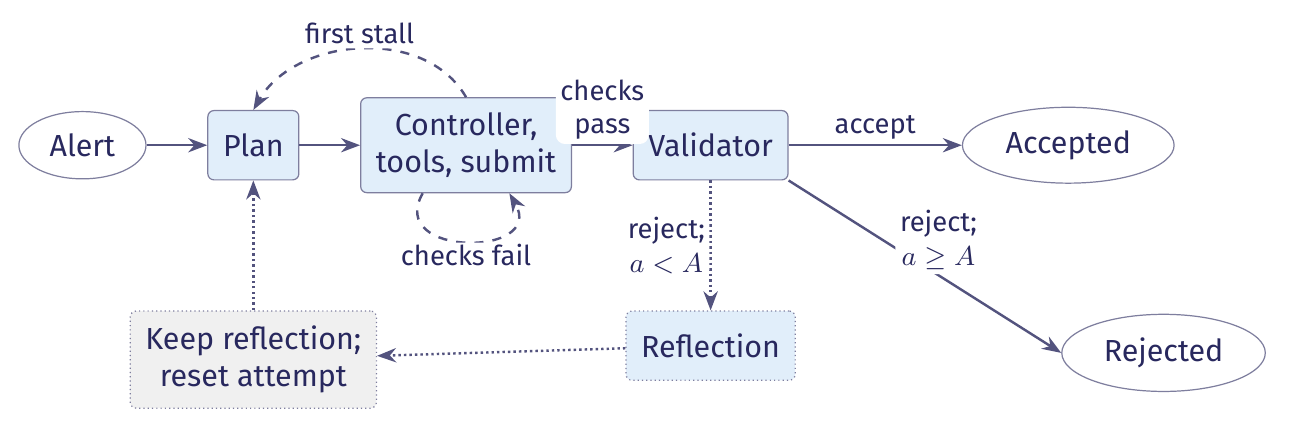
\includegraphics[width=0.78\textwidth]{figures/deck/81a0772b82.png}
  \caption{The proposed feedback edge for new attempts, from the validator back to the plan node.
  A rejection leads to a new attempt while $a$, the number of attempts so far, is below the attempt
  limit $A$, and ends the run otherwise.}
  \label{fig:routing-attempt}
\end{figure*}

After a rejection, the run either writes a reflection, resets the attempt and returns to
\demoref{plan}, or ends, depending on how many attempts it has made. We write $a$ for the value of the attempt
counter and $A$ for the attempt limit. When the validator rejects a patch and $a < A$, the run writes
a reflection and starts a new attempt. When $a \ge A$, the run ends with the status
\demoref{rejected}.

With the new attempt, the plan, the candidate patch and the check results would become attempt
fields, which hold the results of one attempt (\cref{sec:records}). The reset before a new attempt
clears them, so that no later step treats the rejected attempt's results as current. The reflection
survives the reset, and so do the run's counters.

The attempt counter must count attempts across the whole run. If each reset erased it, the counter
would read zero at the start of every attempt, and the runtime could not enforce a limit on the
total number of attempts. The counter therefore has run lifetime, like \demoref{model\_calls}. The
call budget still applies across all attempts.

Every feedback edge must have its own limit or rely on a limit for the whole run. Revision has its
own limit of one per run. Repair and the tool loop rely on the call budget, because both return to
the controller, which either ends the run or makes a model call. The proposed new attempt has both,
the attempt limit and the call budget.

\subsection{Loop bounds and termination}
\label{sec:routing-termination}

A condition for success does not guarantee that a run stops, so termination needs an argument of
its own. The argument answers the question Lecture~2 left open: when do the stopping rules guarantee
that a run ends?

An \textbf{acceptance predicate} is the condition under which a run is declared successful. In the
planning agent, a patch satisfies it when it passes the three submit checks and the validator
accepts it. The \textbf{acceptance procedure} is the code that evaluates the predicate: the submit
checks, followed by the validator's verdict.

A run that never produces an acceptable patch can keep cycling through its feedback edges unless
something else stops it. The acceptance predicate therefore says nothing about whether a run ends.

The usual argument uses a \textbf{loop variant}, a nonnegative integer that decreases on every
continuing cycle \citep{cornell-cs2112-loopinv}. A \textbf{continuing cycle} is one pass around a
loop of the graph, back to the location where it began, after which the run does not end. Because
the variant cannot fall below zero, it bounds the number of cycles. A variant that starts at $n$
allows at most $n$ continuing cycles.

In the planning agent, the variant is $B - c$: the call budget $B$ minus the number $c$ of calls
already made. With our budget of 40, it starts at 40. The argument rests on three conditions:
\bi
\item \textbf{Nonnegative.} The admission check (\cref{sec:records}) keeps $B - c$ nonnegative,
because a node makes a model call only while $c < B$.
\item \textbf{Decreasing.} Every continuing cycle makes at least one model call, so $B - c$ drops by
at least one per cycle.
\item \textbf{Each step returns.} Every step between two model calls returns or times out, so the run
reaches its next model call or its end.
\ei
Under these conditions, a run completes at most $B$ continuing cycles. The conditions bound the
number of cycles. They do not by themselves bound how long a single step takes.

The planning agent meets the decreasing condition. Every loop of its graph passes through the
controller, and a visit to the controller either ends the run or makes a model call. A cycle that
made no model call would leave $B - c$ unchanged, so the budget would not bound it. Such a cycle
needs its own limit. For example, a loop that only reruns tools or checks would need a counter of
its own.

The stall check does not provide a termination argument. It detects identical results. A run whose
tools keep returning different but irrelevant results, for example searches with different patterns
that each find unrelated lines, never triggers it. Such a run can continue without progress until the
budget ends it. Detecting one failure pattern does not prove termination. In our agent, the
termination argument rests on the call budget, provided that every step returns or times out.

Repetition has been observed in reactive agents. ReAct, short for reasoning and acting, is the
pattern that the reactive loop of Lecture~2 follows. In a manual analysis of sampled ReAct
trajectories on a question-answering task, one frequent error pattern was a model that generated its
previous thoughts and actions again and failed to leave the loop \citep[\S3.3]{yao2023react}. Our
stall check detects one consequence of such repetition, identical observations.

The call budget, the stall check and the recursion limit can each end a run before the validator
gives a verdict:
\bi
\item \textbf{The call budget.} Each node that calls a model, namely \demoref{plan},
\demoref{controller} and \demoref{validate}, runs the admission check before it calls the model
(\cref{sec:records}). When
\demoref{model\_calls} has reached the budget of 40, the node returns the status
\demoref{budget\_exhausted} instead of making the call. The check runs before the call, because a
check after the call would let the call incur its cost before the limit was enforced.
\item \textbf{The stall check.} The first stall triggers plan revision (\cref{sec:routing-feedback}).
A second stall, after the revision, ends the run with the status \demoref{no\_progress}.
\item \textbf{The recursion limit.} A \textbf{superstep} is one step of the graph runtime. The
\textbf{recursion limit} caps the number of supersteps in a single run \citep{langgraph-graph-api}.
In our agent it is four times the call budget. It counts supersteps without regard to the task or
to the cost of a step.
\ei

The budget and the recursion limit bound different quantities. The budget counts model calls, which
carry the run's cost. The recursion limit counts supersteps of every kind, so it would also end a
cycle that makes no model call. It would do so only after many supersteps, and it cannot distinguish
a useful step from a wasted one. A cycle without model calls therefore still needs a limit of its
own, tied to what the cycle does.

\subsection{What a trace establishes}
\label{sec:routing-trace}

A trace can establish that a run terminated and that its acceptance procedure passed. No trace event
can establish that the patch is correct. The following claims about a finished run must therefore be
kept apart:
\bi
\item \textbf{Execution stopped.} The \textbf{terminal event} is the event of kind
\demoref{terminal}. It is normally the trace's last event, and its \textbf{terminal status} states
how the run ended. A terminal event establishes that execution terminated.
\item \textbf{Acceptance passed.} A terminal event with the status \demoref{accepted} establishes
that the acceptance procedure passed. The patch passed the submit checks, and the validator accepted
it.
\item \textbf{The patch meets the postcondition.} In the specification of a method, the
\textbf{postcondition} is the implementer's obligation, a condition on the program's state after the
method runs \citep{mit6031-specs}. For a task, it is the condition that the finished artifact, here
the patch, must satisfy. No trace event establishes this claim.
\ei

For our patching task, the postcondition is what Lecture~2's performance measure asks: the weakness
is gone, and the endpoint still behaves as it did. The acceptance procedure produces evidence about
the patch. The submit checks show that the patch applies, touches the flagged line and leaves the
rescan clean.

A clean rescan shows only that the scanner no longer recognizes the flagged pattern (Lecture~2), and
none of the checks runs the endpoint. The validator adds a model's judgment of the patch. Passing
this procedure therefore does not prove that the patch satisfies the postcondition. The trace records
the outcome of the acceptance procedure. It does not establish that the patch is correct.

The model may propose that the work is finished, for example by replying without a tool call. The
submit checks, the validator and the limits then decide how the run ends, and the code of the nodes
sets the terminal status. The validator's verdict comes from a model, but the code of the
\demoref{validate} node turns it into the status \demoref{accepted} or \demoref{rejected}. No model
reply writes the status field directly.

A run of the planning agent ends with one of the following terminal statuses:
\bi
\item \textbf{\demoref{accepted}.} The validator accepted a patch that had passed the submit checks.
\item \textbf{\demoref{rejected}.} The validator rejected the patch.
\item \textbf{\demoref{budget\_exhausted}.} An admission check found the call budget spent before a
model call.
\item \textbf{\demoref{no\_progress}.} The run stalled again after its one plan revision.
\item \textbf{\demoref{error}.} An exception escaped the run.
\ei
The status \demoref{running} marks a run that is still active, so it is never a terminal status.

When a run ends normally, its trace must contain a terminal event. A run ends normally when it
reaches \demoref{END} without an exception. Every exit of the graph sets the status field, and the
runtime records that status in a terminal event before the trace is closed. The trace writer, the
code that appends events to the trace and closes it, checks this rule at closure. If no terminal
event has been written, closing the trace raises an exception that reports a run closed without
stating how it ended.

Every normal ending sets a status, so a terminal event missing at normal closure means that the
recording failed. Such a missing event is an \textbf{instrumentation defect}: a fault in the code
that records the run, which did not record how the run ended.

An escaped exception and a killed process leave different records. If an exception escapes the run,
the trace writer records a terminal event with the status \demoref{error}. It then writes a separate
\demoref{state\_change} event that names the exception, so in this case the terminal event is not
the last event. A
\demoref{SIGKILL} is the operating-system signal that ends a process immediately. The process cannot
intercept it, so none of its code runs after the signal, and no terminal event is written.

\Cref{tab:routing-trace} lists what a reader may conclude from each way a trace can end. The row that
needs the most care is the last one, a trace with no terminal event.

\begin{table}[htbp]
  \caption{What a trace records about the end of a run, and what that record supports.}
  \label{tab:routing-trace}
  \begin{adjustbox}{width=\linewidth}\begin{tabularx}{\linewidth}{L{0.36\linewidth}X}
    \toprule
    \textbf{What the trace records} & \textbf{What it supports} \\
    \midrule
    \textbf{A verdict, then a terminal event with status \demoref{accepted}} & Execution terminated
    and the acceptance procedure passed. The trace does not establish that the patch meets the
    task's postcondition. \\
    \addlinespace
    \textbf{A terminal event with status \demoref{rejected}, \demoref{budget\_exhausted},
    \demoref{no\_progress} or \demoref{error}} & Execution terminated without acceptance, for the
    reason the status states. The events before the ending record how far the run got. For
    \demoref{error}, the next event names the exception. \\
    \addlinespace
    \textbf{No terminal event} & The trace does not establish termination. The run may still be
    active, or the process may have been killed before it could write a terminal event. \\
    \bottomrule
  \end{tabularx}\end{adjustbox}
\end{table}

Labeling a run \demoref{error} because its trace has no terminal event assigns a cause without
evidence. The status \demoref{error} states that an exception escaped the run, and a trace without a
terminal event does not show that. The run may still be active, or it may have been killed. The
accurate reading is that the trace establishes neither whether the run ended nor how.

\subsection{A recorded repair and a keyboard interruption}
\label{sec:routing-recorded}

A second recorded run of the planning agent shows the repair edge taken twice and a run ended by an
interruption. The run worked on a path-traversal alert in OWASP BenchmarkPython, an alert about a
file path that may be built from outside input.

The first patch applied successfully. It left the flagged line unchanged, however, and the rescan
still reported the alert. The trace shows the following sequence:
\bi
\item \textbf{The checks.} The \demoref{submit} node recorded its check results: the patch applies,
it does not touch the flagged line, and the rescan is not clean. It also recorded a reason for each
failed check.
\item \textbf{The routing event.} The next event routed the run to the controller with
\demoref{by} set to \demoref{runtime}, because the tested value was a check result. It stated that
the submit checks had failed and listed both reasons.
\item \textbf{The repair.} The controller received both reasons as a conversation message. It then
ran further rounds through the tools (\cref{sec:machines}) and submitted again.
\ei

The second submission left the rescan clean, but the patch still did not touch the flagged line.
That check failed, the runtime returned its reason to the controller, and the repair edge was taken
a second time.

After more rounds through the tools, a keyboard interrupt stopped the run. A keyboard interrupt is
the signal sent when a user presses Ctrl-C, and Python raises it inside the program as the exception
\demoref{KeyboardInterrupt}. The trace ends with the last tool result, a terminal event with the
status \demoref{error}, and a \demoref{state\_change} event that names the exception. This ending falls in the second row of
\cref{tab:routing-trace}. The trace establishes that execution terminated without acceptance, and it
names the exception. It does not establish what the process was doing between the last tool result
and the interrupt.

A \demoref{SIGKILL} at the same point would have left a different trace. The trace would end at the
last tool result, with neither a terminal event nor the event that names an exception. It would fall in the last
row of \cref{tab:routing-trace}, and it would not establish that the run terminated.

Neither recorded run ended with the status \demoref{budget\_exhausted}. What we have said about that
ending is inferred from the transition rules. No recorded trace shows it.

\subsection*{Key points}
\bi
\item At each visit to a control location that has a routing function, the function tests the merged
record and selects one destination, so one compiled graph can send a run along different paths.
\item The \demoref{by} field of a routing event records whether the model or the runtime supplied the
tested value, and the programmer writes every guard in both cases.
\item For an active run, the routing function after the controller tests only whether the last reply
contains tool calls, so text in a reply that claims the work is finished has no effect on routing.
\item Every feedback edge needs a trigger, the information it passes back and a bound: revision is
limited to one per run, repair by the call budget, and the proposed new attempt by an attempt
counter that survives every reset and by the call budget.
\item An acceptance predicate only defines success, so termination needs a loop variant, here the
budget minus the calls made, which bounds only the cycles that make a model call, so a cycle without
one needs a limit of its own besides the recursion limit, which counts supersteps without regard to
the task, and the stall check, which detects one failure pattern, does not prove termination.
\item A terminal event establishes that a run terminated and the status \demoref{accepted}
establishes that the acceptance procedure passed, while no trace event establishes that the patch
meets the task's postcondition.
\item A trace without a terminal event does not establish termination, because the run may still be
active or its process may have been killed, so labeling such a run \demoref{error} assigns a cause
without evidence.
\ei
